\documentclass[twoside]{book}

% Packages required by doxygen
\usepackage{fixltx2e}
\usepackage{calc}
\usepackage{doxygen}
\usepackage[export]{adjustbox} % also loads graphicx
\usepackage{graphicx}
\usepackage[utf8]{inputenc}
\usepackage{makeidx}
\usepackage{multicol}
\usepackage{multirow}
\PassOptionsToPackage{warn}{textcomp}
\usepackage{textcomp}
\usepackage[nointegrals]{wasysym}
\usepackage[table]{xcolor}

% Font selection
\usepackage[T1]{fontenc}
\usepackage[scaled=.90]{helvet}
\usepackage{courier}
\usepackage{amssymb}
\usepackage{sectsty}
\renewcommand{\familydefault}{\sfdefault}
\allsectionsfont{%
  \fontseries{bc}\selectfont%
  \color{darkgray}%
}
\renewcommand{\DoxyLabelFont}{%
  \fontseries{bc}\selectfont%
  \color{darkgray}%
}
\newcommand{\+}{\discretionary{\mbox{\scriptsize$\hookleftarrow$}}{}{}}

% Page & text layout
\usepackage{geometry}
\geometry{%
  a4paper,%
  top=2.5cm,%
  bottom=2.5cm,%
  left=2.5cm,%
  right=2.5cm%
}
\tolerance=750
\hfuzz=15pt
\hbadness=750
\setlength{\emergencystretch}{15pt}
\setlength{\parindent}{0cm}
\setlength{\parskip}{3ex plus 2ex minus 2ex}
\makeatletter
\renewcommand{\paragraph}{%
  \@startsection{paragraph}{4}{0ex}{-1.0ex}{1.0ex}{%
    \normalfont\normalsize\bfseries\SS@parafont%
  }%
}
\renewcommand{\subparagraph}{%
  \@startsection{subparagraph}{5}{0ex}{-1.0ex}{1.0ex}{%
    \normalfont\normalsize\bfseries\SS@subparafont%
  }%
}
\makeatother

% Headers & footers
\usepackage{fancyhdr}
\pagestyle{fancyplain}
\fancyhead[LE]{\fancyplain{}{\bfseries\thepage}}
\fancyhead[CE]{\fancyplain{}{}}
\fancyhead[RE]{\fancyplain{}{\bfseries\leftmark}}
\fancyhead[LO]{\fancyplain{}{\bfseries\rightmark}}
\fancyhead[CO]{\fancyplain{}{}}
\fancyhead[RO]{\fancyplain{}{\bfseries\thepage}}
\fancyfoot[LE]{\fancyplain{}{}}
\fancyfoot[CE]{\fancyplain{}{}}
\fancyfoot[RE]{\fancyplain{}{\bfseries\scriptsize Generated by Doxygen }}
\fancyfoot[LO]{\fancyplain{}{\bfseries\scriptsize Generated by Doxygen }}
\fancyfoot[CO]{\fancyplain{}{}}
\fancyfoot[RO]{\fancyplain{}{}}
\renewcommand{\footrulewidth}{0.4pt}
\renewcommand{\chaptermark}[1]{%
  \markboth{#1}{}%
}
\renewcommand{\sectionmark}[1]{%
  \markright{\thesection\ #1}%
}

% Indices & bibliography
\usepackage{natbib}
\usepackage[titles]{tocloft}
\setcounter{tocdepth}{3}
\setcounter{secnumdepth}{5}
\makeindex

% Hyperlinks (required, but should be loaded last)
\usepackage{ifpdf}
\ifpdf
  \usepackage[pdftex,pagebackref=true]{hyperref}
\else
  \usepackage[ps2pdf,pagebackref=true]{hyperref}
\fi
\hypersetup{%
  colorlinks=true,%
  linkcolor=blue,%
  citecolor=blue,%
  unicode%
}

% Custom commands
\newcommand{\clearemptydoublepage}{%
  \newpage{\pagestyle{empty}\cleardoublepage}%
}

\usepackage{caption}
\captionsetup{labelsep=space,justification=centering,font={bf},singlelinecheck=off,skip=4pt,position=top}

%===== C O N T E N T S =====

\begin{document}

% Titlepage & ToC
\hypersetup{pageanchor=false,
             bookmarksnumbered=true,
             pdfencoding=unicode
            }
\pagenumbering{roman}
\begin{titlepage}
\vspace*{7cm}
\begin{center}%
{\Large Crafter }\\
\vspace*{1cm}
{\large Generated by Doxygen 1.8.11}\\
\end{center}
\end{titlepage}
\clearemptydoublepage
\tableofcontents
\clearemptydoublepage
\pagenumbering{arabic}
\hypersetup{pageanchor=true}

%--- Begin generated contents ---
\chapter{Modelling Utility}
\label{index}\hypertarget{index}{}This program is capable of creating raw models. Models are to be made using Modeling mode. While modeing Color could be selected using color palatte and triangle can be drawn of the selected color. The inspection mode has features such as recentering about the centroid for viewing what has been modeled. The program also saves model in raw format and could load it for later use. Undo commands removes the last add vertices. Multiple use of undo retraces the history of how the Model was created. 
\chapter{Class Index}
\section{Class List}
Here are the classes, structs, unions and interfaces with brief descriptions\+:\begin{DoxyCompactList}
\item\contentsline{section}{\hyperlink{classcft_1_1Crafter}{cft\+::\+Crafter} \\*Class that is basically the main program }{\pageref{classcft_1_1Crafter}}{}
\item\contentsline{section}{\hyperlink{classcft_1_1Model}{cft\+::\+Model} \\*Class that is abstraction of a 3\+D-\/\+Model }{\pageref{classcft_1_1Model}}{}
\item\contentsline{section}{\hyperlink{classcft_1_1Palette}{cft\+::\+Palette} \\*Class that displays a Rectangle Color-\/\+Palette to choose from }{\pageref{classcft_1_1Palette}}{}
\item\contentsline{section}{\hyperlink{classcft_1_1Scene}{cft\+::\+Scene} \\*Class that is basically the main program }{\pageref{classcft_1_1Scene}}{}
\end{DoxyCompactList}

\chapter{File Index}
\section{File List}
Here is a list of all documented files with brief descriptions\+:\begin{DoxyCompactList}
\item\contentsline{section}{\hyperlink{config_8hpp}{config.\+hpp} \\*This stores all constants required to run the Crafter for simplicity of modifying }{\pageref{config_8hpp}}{}
\item\contentsline{section}{\hyperlink{crafter_8hpp}{crafter.\+hpp} \\*Class declaration for the program managing the state and models }{\pageref{crafter_8hpp}}{}
\item\contentsline{section}{\hyperlink{Main_8cpp}{Main.\+cpp} \\*Main funciton which creates and passes the window to the Crafter }{\pageref{Main_8cpp}}{}
\item\contentsline{section}{\hyperlink{model_8hpp}{model.\+hpp} \\*Class declaration for the Model }{\pageref{model_8hpp}}{}
\item\contentsline{section}{\hyperlink{palette_8hpp}{palette.\+hpp} \\*Class declaration for the Color Palette }{\pageref{palette_8hpp}}{}
\item\contentsline{section}{{\bfseries shader\+\_\+util.\+hpp} }{\pageref{shader__util_8hpp}}{}
\end{DoxyCompactList}

\chapter{Class Documentation}
\hypertarget{classcft_1_1Crafter}{}\section{cft\+:\+:Crafter Class Reference}
\label{classcft_1_1Crafter}\index{cft\+::\+Crafter@{cft\+::\+Crafter}}


Class that is basically the main program.  




{\ttfamily \#include $<$crafter.\+hpp$>$}



Collaboration diagram for cft\+:\+:Crafter\+:
% FIG 0
\subsection*{Public Member Functions}
\begin{DoxyCompactItemize}
\item 
\hyperlink{classcft_1_1Crafter_a57796fe2de2fe073c8a7ef14e2a57d21}{Crafter} ()\hypertarget{classcft_1_1Crafter_a57796fe2de2fe073c8a7ef14e2a57d21}{}\label{classcft_1_1Crafter_a57796fe2de2fe073c8a7ef14e2a57d21}

\begin{DoxyCompactList}\small\item\em Empty constructor should be made private to force to use overloaded constructor. \end{DoxyCompactList}\item 
void \hyperlink{classcft_1_1Crafter_a0e56cb6de077230dfbc29dac9adace2a}{Init} (G\+L\+F\+Wwindow $\ast$\hyperlink{classcft_1_1Crafter_a70b8292b32d9eda7b3ce9e8c86161042}{window})\hypertarget{classcft_1_1Crafter_a0e56cb6de077230dfbc29dac9adace2a}{}\label{classcft_1_1Crafter_a0e56cb6de077230dfbc29dac9adace2a}

\begin{DoxyCompactList}\small\item\em Initializes all the buffers and variables and set the handlers. \end{DoxyCompactList}\item 
void \hyperlink{classcft_1_1Crafter_ad08567005970bdd4b33c2d3816ba4e5d}{Update} ()\hypertarget{classcft_1_1Crafter_ad08567005970bdd4b33c2d3816ba4e5d}{}\label{classcft_1_1Crafter_ad08567005970bdd4b33c2d3816ba4e5d}

\begin{DoxyCompactList}\small\item\em Updates all the variable and state and sets the matrices accordingly. \end{DoxyCompactList}\item 
void \hyperlink{classcft_1_1Crafter_a018462b2e4daf890ac697acbbc1f14d3}{Render} ()\hypertarget{classcft_1_1Crafter_a018462b2e4daf890ac697acbbc1f14d3}{}\label{classcft_1_1Crafter_a018462b2e4daf890ac697acbbc1f14d3}

\begin{DoxyCompactList}\small\item\em Renders the grid, pallete and model in modelling mode and only model in inspection mode. \end{DoxyCompactList}\end{DoxyCompactItemize}
\subsection*{Private Attributes}
\begin{DoxyCompactItemize}
\item 
G\+L\+F\+Wwindow $\ast$ \hyperlink{classcft_1_1Crafter_a70b8292b32d9eda7b3ce9e8c86161042}{window}\hypertarget{classcft_1_1Crafter_a70b8292b32d9eda7b3ce9e8c86161042}{}\label{classcft_1_1Crafter_a70b8292b32d9eda7b3ce9e8c86161042}

\begin{DoxyCompactList}\small\item\em Store the handle for G\+L\+FW Window. \end{DoxyCompactList}\item 
G\+Luint \hyperlink{classcft_1_1Crafter_a9c0adedc2bd7aeb3a1415eb47ea11e04}{shader\+Program}\hypertarget{classcft_1_1Crafter_a9c0adedc2bd7aeb3a1415eb47ea11e04}{}\label{classcft_1_1Crafter_a9c0adedc2bd7aeb3a1415eb47ea11e04}

\begin{DoxyCompactList}\small\item\em Store the handle for shader program. \end{DoxyCompactList}\item 
G\+Luint \hyperlink{classcft_1_1Crafter_a4d5ce47319d35e5e4978bc19682fea6d}{u\+Model\+View\+Matrix}\hypertarget{classcft_1_1Crafter_a4d5ce47319d35e5e4978bc19682fea6d}{}\label{classcft_1_1Crafter_a4d5ce47319d35e5e4978bc19682fea6d}

\begin{DoxyCompactList}\small\item\em Pointer pointing to modeling matrix in the shader. \end{DoxyCompactList}\item 
\hyperlink{classcft_1_1Model}{Model} $\ast$ \hyperlink{classcft_1_1Crafter_a42504406d07a4114368ffdcf6de2b33f}{model}\hypertarget{classcft_1_1Crafter_a42504406d07a4114368ffdcf6de2b33f}{}\label{classcft_1_1Crafter_a42504406d07a4114368ffdcf6de2b33f}

\begin{DoxyCompactList}\small\item\em The current model in focus. \end{DoxyCompactList}\item 
\hyperlink{classcft_1_1Palette}{Palette} $\ast$ \hyperlink{classcft_1_1Crafter_a358b5590166bf9ed437462a922b806f5}{palette}\hypertarget{classcft_1_1Crafter_a358b5590166bf9ed437462a922b806f5}{}\label{classcft_1_1Crafter_a358b5590166bf9ed437462a922b806f5}

\begin{DoxyCompactList}\small\item\em Color palette to choose color from. \end{DoxyCompactList}\end{DoxyCompactItemize}
{\bf }\par
\begin{DoxyCompactItemize}
\item 
G\+Luint \hyperlink{classcft_1_1Crafter_a3770da487be185aaf19b8946998e45fb}{vbo}\hypertarget{classcft_1_1Crafter_a3770da487be185aaf19b8946998e45fb}{}\label{classcft_1_1Crafter_a3770da487be185aaf19b8946998e45fb}

\begin{DoxyCompactList}\small\item\em The vertex buffer and array buffers which stores the vertices of the model and other references. \end{DoxyCompactList}\item 
G\+Luint \hyperlink{classcft_1_1Crafter_aca03f78f43b66c8e1196fbcf19a4b844}{vao}\hypertarget{classcft_1_1Crafter_aca03f78f43b66c8e1196fbcf19a4b844}{}\label{classcft_1_1Crafter_aca03f78f43b66c8e1196fbcf19a4b844}

\begin{DoxyCompactList}\small\item\em The vertex buffer and array buffers which stores the vertices of the model and other references. \end{DoxyCompactList}\end{DoxyCompactItemize}

{\bf }\par
\begin{DoxyCompactItemize}
\item 
glm\+::vec4 \hyperlink{classcft_1_1Crafter_afcc8528696d7bf63d8e5a4a9f05dce55}{vertices} \mbox{[}3\mbox{]}\hypertarget{classcft_1_1Crafter_afcc8528696d7bf63d8e5a4a9f05dce55}{}\label{classcft_1_1Crafter_afcc8528696d7bf63d8e5a4a9f05dce55}

\begin{DoxyCompactList}\small\item\em Variable for displaying points marked on the screen during modeling mode. \end{DoxyCompactList}\item 
glm\+::vec4 \hyperlink{classcft_1_1Crafter_ac05469c2f55a2988e145225a2d982292}{color} \mbox{[}3\mbox{]}\hypertarget{classcft_1_1Crafter_ac05469c2f55a2988e145225a2d982292}{}\label{classcft_1_1Crafter_ac05469c2f55a2988e145225a2d982292}

\begin{DoxyCompactList}\small\item\em Variable for displaying points marked on the screen during modeling mode. \end{DoxyCompactList}\item 
glm\+::vec4 $\ast$ \hyperlink{classcft_1_1Crafter_a4c305e74e5e73b9a29a54d4f3d2a27ee}{points}\hypertarget{classcft_1_1Crafter_a4c305e74e5e73b9a29a54d4f3d2a27ee}{}\label{classcft_1_1Crafter_a4c305e74e5e73b9a29a54d4f3d2a27ee}

\begin{DoxyCompactList}\small\item\em Variable for displaying points marked on the screen during modeling mode. \end{DoxyCompactList}\item 
glm\+::vec4 $\ast$ \hyperlink{classcft_1_1Crafter_a57ad393984170475d18f64af191ba414}{point\+\_\+color}\hypertarget{classcft_1_1Crafter_a57ad393984170475d18f64af191ba414}{}\label{classcft_1_1Crafter_a57ad393984170475d18f64af191ba414}

\begin{DoxyCompactList}\small\item\em Variable for displaying points marked on the screen during modeling mode. \end{DoxyCompactList}\item 
int \hyperlink{classcft_1_1Crafter_af938d739229975ec35d64ee76e683bc4}{state}\hypertarget{classcft_1_1Crafter_af938d739229975ec35d64ee76e683bc4}{}\label{classcft_1_1Crafter_af938d739229975ec35d64ee76e683bc4}

\begin{DoxyCompactList}\small\item\em Varible for displaying the grid during the Modelling mode. \end{DoxyCompactList}\item 
int \hyperlink{classcft_1_1Crafter_a1302b2d0ab7a24b60eb27d7c2178dc9a}{index}\hypertarget{classcft_1_1Crafter_a1302b2d0ab7a24b60eb27d7c2178dc9a}{}\label{classcft_1_1Crafter_a1302b2d0ab7a24b60eb27d7c2178dc9a}

\begin{DoxyCompactList}\small\item\em Variable for displaying points marked on the screen during modeling mode. \end{DoxyCompactList}\item 
int \hyperlink{classcft_1_1Crafter_a33c6d9e2708e21497d8318f0b7de0ba4}{total\+\_\+lines}\hypertarget{classcft_1_1Crafter_a33c6d9e2708e21497d8318f0b7de0ba4}{}\label{classcft_1_1Crafter_a33c6d9e2708e21497d8318f0b7de0ba4}

\begin{DoxyCompactList}\small\item\em Variable for displaying points marked on the screen during modeling mode. \end{DoxyCompactList}\item 
int \hyperlink{classcft_1_1Crafter_a7bff56ecf0bb45110088f9158410eeab}{total\+\_\+points}\hypertarget{classcft_1_1Crafter_a7bff56ecf0bb45110088f9158410eeab}{}\label{classcft_1_1Crafter_a7bff56ecf0bb45110088f9158410eeab}

\begin{DoxyCompactList}\small\item\em Variable for displaying points marked on the screen during modeling mode. \end{DoxyCompactList}\end{DoxyCompactItemize}

\begin{DoxyCompactItemize}
\item 
static bool \hyperlink{classcft_1_1Crafter_ab9c026d68e1732d7dc21259dcad3cd1c}{key\+\_\+up} = false\hypertarget{classcft_1_1Crafter_ab9c026d68e1732d7dc21259dcad3cd1c}{}\label{classcft_1_1Crafter_ab9c026d68e1732d7dc21259dcad3cd1c}

\begin{DoxyCompactList}\small\item\em Handlers are static as non static member functions couldn\textquotesingle{}t be passed as arguments so are the variable storing the state. \end{DoxyCompactList}\item 
static bool \hyperlink{classcft_1_1Crafter_a19722ca805f96abccf36377a6806be11}{key\+\_\+down} = false\hypertarget{classcft_1_1Crafter_a19722ca805f96abccf36377a6806be11}{}\label{classcft_1_1Crafter_a19722ca805f96abccf36377a6806be11}

\begin{DoxyCompactList}\small\item\em Handlers are static as non static member functions couldn\textquotesingle{}t be passed as arguments so are the variable storing the state. \end{DoxyCompactList}\item 
static bool \hyperlink{classcft_1_1Crafter_a0ed59897a463c72fbd32dc18a92996f3}{key\+\_\+left} = false\hypertarget{classcft_1_1Crafter_a0ed59897a463c72fbd32dc18a92996f3}{}\label{classcft_1_1Crafter_a0ed59897a463c72fbd32dc18a92996f3}

\begin{DoxyCompactList}\small\item\em Handlers are static as non static member functions couldn\textquotesingle{}t be passed as arguments so are the variable storing the state. \end{DoxyCompactList}\item 
static bool \hyperlink{classcft_1_1Crafter_a82b154c79774e330a091f8b900cffe6e}{key\+\_\+right} = false\hypertarget{classcft_1_1Crafter_a82b154c79774e330a091f8b900cffe6e}{}\label{classcft_1_1Crafter_a82b154c79774e330a091f8b900cffe6e}

\begin{DoxyCompactList}\small\item\em Handlers are static as non static member functions couldn\textquotesingle{}t be passed as arguments so are the variable storing the state. \end{DoxyCompactList}\item 
static bool \hyperlink{classcft_1_1Crafter_ad3cd666334f96bdae838c493f555f4bf}{key\+\_\+M} = false\hypertarget{classcft_1_1Crafter_ad3cd666334f96bdae838c493f555f4bf}{}\label{classcft_1_1Crafter_ad3cd666334f96bdae838c493f555f4bf}

\begin{DoxyCompactList}\small\item\em Handlers are static as non static member functions couldn\textquotesingle{}t be passed as arguments so are the variable storing the state. \end{DoxyCompactList}\item 
static bool \hyperlink{classcft_1_1Crafter_afe83086cdb6ea720b2126d642e4018fe}{key\+\_\+I} = false\hypertarget{classcft_1_1Crafter_afe83086cdb6ea720b2126d642e4018fe}{}\label{classcft_1_1Crafter_afe83086cdb6ea720b2126d642e4018fe}

\begin{DoxyCompactList}\small\item\em Handlers are static as non static member functions couldn\textquotesingle{}t be passed as arguments so are the variable storing the state. \end{DoxyCompactList}\item 
static bool \hyperlink{classcft_1_1Crafter_ae28043611771b66238001adb88466b2d}{key\+\_\+L} = false\hypertarget{classcft_1_1Crafter_ae28043611771b66238001adb88466b2d}{}\label{classcft_1_1Crafter_ae28043611771b66238001adb88466b2d}

\begin{DoxyCompactList}\small\item\em Handlers are static as non static member functions couldn\textquotesingle{}t be passed as arguments so are the variable storing the state. \end{DoxyCompactList}\item 
static bool \hyperlink{classcft_1_1Crafter_a66d84d75359750f76edc2e57cacd0e17}{key\+\_\+K} = false\hypertarget{classcft_1_1Crafter_a66d84d75359750f76edc2e57cacd0e17}{}\label{classcft_1_1Crafter_a66d84d75359750f76edc2e57cacd0e17}

\begin{DoxyCompactList}\small\item\em Handlers are static as non static member functions couldn\textquotesingle{}t be passed as arguments so are the variable storing the state. \end{DoxyCompactList}\item 
static bool \hyperlink{classcft_1_1Crafter_ac55c5f1123a89784119179de05b1db99}{key\+\_\+R} = false\hypertarget{classcft_1_1Crafter_ac55c5f1123a89784119179de05b1db99}{}\label{classcft_1_1Crafter_ac55c5f1123a89784119179de05b1db99}

\begin{DoxyCompactList}\small\item\em Handlers are static as non static member functions couldn\textquotesingle{}t be passed as arguments so are the variable storing the state. \end{DoxyCompactList}\item 
static bool \hyperlink{classcft_1_1Crafter_ae75a4e2b8670355dd0a008f79297efad}{key\+\_\+W} = false\hypertarget{classcft_1_1Crafter_ae75a4e2b8670355dd0a008f79297efad}{}\label{classcft_1_1Crafter_ae75a4e2b8670355dd0a008f79297efad}

\begin{DoxyCompactList}\small\item\em Handlers are static as non static member functions couldn\textquotesingle{}t be passed as arguments so are the variable storing the state. \end{DoxyCompactList}\item 
static bool \hyperlink{classcft_1_1Crafter_a5d9a03f72de437086e9beb2dffd39cca}{key\+\_\+A} = false\hypertarget{classcft_1_1Crafter_a5d9a03f72de437086e9beb2dffd39cca}{}\label{classcft_1_1Crafter_a5d9a03f72de437086e9beb2dffd39cca}

\begin{DoxyCompactList}\small\item\em Handlers are static as non static member functions couldn\textquotesingle{}t be passed as arguments so are the variable storing the state. \end{DoxyCompactList}\item 
static bool \hyperlink{classcft_1_1Crafter_ae8d219172097605d7511564e6a7c4236}{key\+\_\+S} = false\hypertarget{classcft_1_1Crafter_ae8d219172097605d7511564e6a7c4236}{}\label{classcft_1_1Crafter_ae8d219172097605d7511564e6a7c4236}

\begin{DoxyCompactList}\small\item\em Handlers are static as non static member functions couldn\textquotesingle{}t be passed as arguments so are the variable storing the state. \end{DoxyCompactList}\item 
static bool \hyperlink{classcft_1_1Crafter_a1b25b4753e092c47dd1557d4583caaa9}{key\+\_\+D} = false\hypertarget{classcft_1_1Crafter_a1b25b4753e092c47dd1557d4583caaa9}{}\label{classcft_1_1Crafter_a1b25b4753e092c47dd1557d4583caaa9}

\begin{DoxyCompactList}\small\item\em Handlers are static as non static member functions couldn\textquotesingle{}t be passed as arguments so are the variable storing the state. \end{DoxyCompactList}\item 
static bool \hyperlink{classcft_1_1Crafter_aa2c40e67f2e7267a1e250b33102034b7}{key\+\_\+Z} = false\hypertarget{classcft_1_1Crafter_aa2c40e67f2e7267a1e250b33102034b7}{}\label{classcft_1_1Crafter_aa2c40e67f2e7267a1e250b33102034b7}

\begin{DoxyCompactList}\small\item\em Handlers are static as non static member functions couldn\textquotesingle{}t be passed as arguments so are the variable storing the state. \end{DoxyCompactList}\item 
static bool \hyperlink{classcft_1_1Crafter_a89c9924a417a474455da1e5d0b6ac9ce}{key\+\_\+X} = false\hypertarget{classcft_1_1Crafter_a89c9924a417a474455da1e5d0b6ac9ce}{}\label{classcft_1_1Crafter_a89c9924a417a474455da1e5d0b6ac9ce}

\begin{DoxyCompactList}\small\item\em Handlers are static as non static member functions couldn\textquotesingle{}t be passed as arguments so are the variable storing the state. \end{DoxyCompactList}\item 
static bool \hyperlink{classcft_1_1Crafter_a92f23c00adff2309b06545cb7a524d68}{key\+\_\+\+Pg\+Up} = false\hypertarget{classcft_1_1Crafter_a92f23c00adff2309b06545cb7a524d68}{}\label{classcft_1_1Crafter_a92f23c00adff2309b06545cb7a524d68}

\begin{DoxyCompactList}\small\item\em Handlers are static as non static member functions couldn\textquotesingle{}t be passed as arguments so are the variable storing the state. \end{DoxyCompactList}\item 
static bool \hyperlink{classcft_1_1Crafter_a7f78d9d9a708cfb5f0ce1b4d21721702}{key\+\_\+\+Pg\+Down} = false\hypertarget{classcft_1_1Crafter_a7f78d9d9a708cfb5f0ce1b4d21721702}{}\label{classcft_1_1Crafter_a7f78d9d9a708cfb5f0ce1b4d21721702}

\begin{DoxyCompactList}\small\item\em Handlers are static as non static member functions couldn\textquotesingle{}t be passed as arguments so are the variable storing the state. \end{DoxyCompactList}\item 
static bool \hyperlink{classcft_1_1Crafter_ae97908b05847ba781d3ba8144b085d7b}{key\+\_\+shift} = false\hypertarget{classcft_1_1Crafter_ae97908b05847ba781d3ba8144b085d7b}{}\label{classcft_1_1Crafter_ae97908b05847ba781d3ba8144b085d7b}

\begin{DoxyCompactList}\small\item\em Handlers are static as non static member functions couldn\textquotesingle{}t be passed as arguments so are the variable storing the state. \end{DoxyCompactList}\item 
static bool \hyperlink{classcft_1_1Crafter_a4cd46febce4662a475ce4731c40e3763}{key\+\_\+1} = false\hypertarget{classcft_1_1Crafter_a4cd46febce4662a475ce4731c40e3763}{}\label{classcft_1_1Crafter_a4cd46febce4662a475ce4731c40e3763}

\begin{DoxyCompactList}\small\item\em Handlers are static as non static member functions couldn\textquotesingle{}t be passed as arguments so are the variable storing the state. \end{DoxyCompactList}\item 
static bool \hyperlink{classcft_1_1Crafter_a084a0fd701eabdf854d17c62281e3e9f}{key\+\_\+2} = false\hypertarget{classcft_1_1Crafter_a084a0fd701eabdf854d17c62281e3e9f}{}\label{classcft_1_1Crafter_a084a0fd701eabdf854d17c62281e3e9f}

\begin{DoxyCompactList}\small\item\em Handlers are static as non static member functions couldn\textquotesingle{}t be passed as arguments so are the variable storing the state. \end{DoxyCompactList}\item 
static bool \hyperlink{classcft_1_1Crafter_aaa2687d319fd3ad3b7e27f80298d9ea8}{key\+\_\+3} = false\hypertarget{classcft_1_1Crafter_aaa2687d319fd3ad3b7e27f80298d9ea8}{}\label{classcft_1_1Crafter_aaa2687d319fd3ad3b7e27f80298d9ea8}

\begin{DoxyCompactList}\small\item\em Handlers are static as non static member functions couldn\textquotesingle{}t be passed as arguments so are the variable storing the state. \end{DoxyCompactList}\item 
static bool \hyperlink{classcft_1_1Crafter_af67075057122adcf1e6d25ebe5cb9142}{key\+\_\+4} = false\hypertarget{classcft_1_1Crafter_af67075057122adcf1e6d25ebe5cb9142}{}\label{classcft_1_1Crafter_af67075057122adcf1e6d25ebe5cb9142}

\begin{DoxyCompactList}\small\item\em Handlers are static as non static member functions couldn\textquotesingle{}t be passed as arguments so are the variable storing the state. \end{DoxyCompactList}\item 
static bool \hyperlink{classcft_1_1Crafter_aec1e3274567e07538fff997f19322c41}{key\+\_\+5} = false\hypertarget{classcft_1_1Crafter_aec1e3274567e07538fff997f19322c41}{}\label{classcft_1_1Crafter_aec1e3274567e07538fff997f19322c41}

\begin{DoxyCompactList}\small\item\em Handlers are static as non static member functions couldn\textquotesingle{}t be passed as arguments so are the variable storing the state. \end{DoxyCompactList}\item 
static bool \hyperlink{classcft_1_1Crafter_a2f81f98cb113930587877ee178a916d4}{key\+\_\+6} = false\hypertarget{classcft_1_1Crafter_a2f81f98cb113930587877ee178a916d4}{}\label{classcft_1_1Crafter_a2f81f98cb113930587877ee178a916d4}

\begin{DoxyCompactList}\small\item\em Handlers are static as non static member functions couldn\textquotesingle{}t be passed as arguments so are the variable storing the state. \end{DoxyCompactList}\item 
static bool \hyperlink{classcft_1_1Crafter_a1e09ec121632860c6f8eaf7439eca600}{button\+\_\+left} = false\hypertarget{classcft_1_1Crafter_a1e09ec121632860c6f8eaf7439eca600}{}\label{classcft_1_1Crafter_a1e09ec121632860c6f8eaf7439eca600}

\begin{DoxyCompactList}\small\item\em Handlers are static as non static member functions couldn\textquotesingle{}t be passed as arguments so are the variable storing the state. \end{DoxyCompactList}\item 
static double \hyperlink{classcft_1_1Crafter_a5c2adcdf34e2dd99cefc0ae9d8ad6af0}{posx} = 0\hypertarget{classcft_1_1Crafter_a5c2adcdf34e2dd99cefc0ae9d8ad6af0}{}\label{classcft_1_1Crafter_a5c2adcdf34e2dd99cefc0ae9d8ad6af0}

\begin{DoxyCompactList}\small\item\em Handlers are static as non static member functions couldn\textquotesingle{}t be passed as arguments so are the variable storing the state. \end{DoxyCompactList}\item 
static double \hyperlink{classcft_1_1Crafter_a1ddfd1c078cfee931cdf01f66bfee489}{posy} = 0\hypertarget{classcft_1_1Crafter_a1ddfd1c078cfee931cdf01f66bfee489}{}\label{classcft_1_1Crafter_a1ddfd1c078cfee931cdf01f66bfee489}

\begin{DoxyCompactList}\small\item\em Handlers are static as non static member functions couldn\textquotesingle{}t be passed as arguments so are the variable storing the state. \end{DoxyCompactList}\item 
static double \hyperlink{classcft_1_1Crafter_a18a6178af00edeb349988756322db7a4}{posz} = screen\+\_\+depth/2\hypertarget{classcft_1_1Crafter_a18a6178af00edeb349988756322db7a4}{}\label{classcft_1_1Crafter_a18a6178af00edeb349988756322db7a4}

\begin{DoxyCompactList}\small\item\em Handlers are static as non static member functions couldn\textquotesingle{}t be passed as arguments so are the variable storing the state. \end{DoxyCompactList}\item 
static int \hyperlink{classcft_1_1Crafter_a6d2febc7e21fc2c197a4d7d0b3558d96}{col\+\_\+r} = 128\hypertarget{classcft_1_1Crafter_a6d2febc7e21fc2c197a4d7d0b3558d96}{}\label{classcft_1_1Crafter_a6d2febc7e21fc2c197a4d7d0b3558d96}

\begin{DoxyCompactList}\small\item\em Handlers are static as non static member functions couldn\textquotesingle{}t be passed as arguments so are the variable storing the state. \end{DoxyCompactList}\item 
static int \hyperlink{classcft_1_1Crafter_af2635f8b801c0fc7b51445da759c4523}{col\+\_\+g} = 128\hypertarget{classcft_1_1Crafter_af2635f8b801c0fc7b51445da759c4523}{}\label{classcft_1_1Crafter_af2635f8b801c0fc7b51445da759c4523}

\begin{DoxyCompactList}\small\item\em Handlers are static as non static member functions couldn\textquotesingle{}t be passed as arguments so are the variable storing the state. \end{DoxyCompactList}\item 
static int \hyperlink{classcft_1_1Crafter_a69402d955cc6a8ab59ae82f74c52eb88}{col\+\_\+b} = 128\hypertarget{classcft_1_1Crafter_a69402d955cc6a8ab59ae82f74c52eb88}{}\label{classcft_1_1Crafter_a69402d955cc6a8ab59ae82f74c52eb88}

\begin{DoxyCompactList}\small\item\em Handlers are static as non static member functions couldn\textquotesingle{}t be passed as arguments so are the variable storing the state. \end{DoxyCompactList}\item 
static void \hyperlink{classcft_1_1Crafter_a41f99673082ebc4b26b5c844f106a870}{Keyboard\+Handler} (G\+L\+F\+Wwindow $\ast$\hyperlink{classcft_1_1Crafter_a70b8292b32d9eda7b3ce9e8c86161042}{window}, int key, int scancode, int action, int mods)\hypertarget{classcft_1_1Crafter_a41f99673082ebc4b26b5c844f106a870}{}\label{classcft_1_1Crafter_a41f99673082ebc4b26b5c844f106a870}

\begin{DoxyCompactList}\small\item\em Handlers are static as non static member functions couldn\textquotesingle{}t be passed as arguments so are the variable storing the state. \end{DoxyCompactList}\item 
static void \hyperlink{classcft_1_1Crafter_acc54c5bd962b9c7a259a76589052e08e}{Mouse\+Handler} (G\+L\+F\+Wwindow $\ast$\hyperlink{classcft_1_1Crafter_a70b8292b32d9eda7b3ce9e8c86161042}{window}, int button, int action, int mods)\hypertarget{classcft_1_1Crafter_acc54c5bd962b9c7a259a76589052e08e}{}\label{classcft_1_1Crafter_acc54c5bd962b9c7a259a76589052e08e}

\begin{DoxyCompactList}\small\item\em Handlers are static as non static member functions couldn\textquotesingle{}t be passed as arguments so are the variable storing the state. \end{DoxyCompactList}\item 
static void \hyperlink{classcft_1_1Crafter_a95820140f31bbea4f9aa2d70bf2bc9a1}{Cursor\+Handler} (G\+L\+F\+Wwindow $\ast$\hyperlink{classcft_1_1Crafter_a70b8292b32d9eda7b3ce9e8c86161042}{window}, double x, double y)\hypertarget{classcft_1_1Crafter_a95820140f31bbea4f9aa2d70bf2bc9a1}{}\label{classcft_1_1Crafter_a95820140f31bbea4f9aa2d70bf2bc9a1}

\begin{DoxyCompactList}\small\item\em Handlers are static as non static member functions couldn\textquotesingle{}t be passed as arguments so are the variable storing the state. \end{DoxyCompactList}\item 
static void \hyperlink{classcft_1_1Crafter_ac3a3d9f8dca115508e85f38c9e66eee5}{Resize\+Handler} (G\+L\+F\+Wwindow $\ast$\hyperlink{classcft_1_1Crafter_a70b8292b32d9eda7b3ce9e8c86161042}{window}, int width, int height)\hypertarget{classcft_1_1Crafter_ac3a3d9f8dca115508e85f38c9e66eee5}{}\label{classcft_1_1Crafter_ac3a3d9f8dca115508e85f38c9e66eee5}

\begin{DoxyCompactList}\small\item\em Handlers are static as non static member functions couldn\textquotesingle{}t be passed as arguments so are the variable storing the state. \end{DoxyCompactList}\item 
static void \hyperlink{classcft_1_1Crafter_ad145c5077488de420916468c97a638e8}{Error\+Handler} (int error, const char $\ast$description)\hypertarget{classcft_1_1Crafter_ad145c5077488de420916468c97a638e8}{}\label{classcft_1_1Crafter_ad145c5077488de420916468c97a638e8}

\begin{DoxyCompactList}\small\item\em Handlers are static as non static member functions couldn\textquotesingle{}t be passed as arguments so are the variable storing the state. \end{DoxyCompactList}\end{DoxyCompactItemize}


\subsection{Detailed Description}
Class that is basically the main program. 

This class has various input handler and hand various functions changing state variables accordingly. State variable defines the behaviour of the rendering and modification of the model or loading and saving of the model. It has two modes Modelling and Inspection modes. Modelling mode lets you create model by generating vertices. Inspection lets you view your model in perspective projection 

The documentation for this class was generated from the following files\+:\begin{DoxyCompactItemize}
\item 
\hyperlink{crafter_8hpp}{crafter.\+hpp}\item 
crafter.\+cpp\end{DoxyCompactItemize}

\hypertarget{classcft_1_1Model}{}\section{cft\+:\+:Model Class Reference}
\label{classcft_1_1Model}\index{cft\+::\+Model@{cft\+::\+Model}}


Class that is abstraction of a 3\+D-\/\+Model.  




{\ttfamily \#include $<$model.\+hpp$>$}

\subsection*{Public Member Functions}
\begin{DoxyCompactItemize}
\item 
\hyperlink{classcft_1_1Model_a3c0c1f66829e59fcab5786aac5086a4a}{Model} ()\hypertarget{classcft_1_1Model_a3c0c1f66829e59fcab5786aac5086a4a}{}\label{classcft_1_1Model_a3c0c1f66829e59fcab5786aac5086a4a}

\begin{DoxyCompactList}\small\item\em Empty Constructor. \end{DoxyCompactList}\item 
\hyperlink{classcft_1_1Model_a1f3e508bf9546bc63970d2f9386093eb}{Model} (G\+Luint shader\+Program)
\begin{DoxyCompactList}\small\item\em Overloaded constructor of the object. \end{DoxyCompactList}\item 
void \hyperlink{classcft_1_1Model_a1f200fd7be2eee7ef2c7932d9fa62fc9}{Load\+Model} (std\+::string file)
\begin{DoxyCompactList}\small\item\em Loads all the vertices of the model in a file. \end{DoxyCompactList}\item 
void \hyperlink{classcft_1_1Model_ac1c81c55d6a29bfedaa156a65334b525}{Save\+Model} (std\+::string file)
\begin{DoxyCompactList}\small\item\em Stores all the vertices of the model in a file. \end{DoxyCompactList}\item 
void \hyperlink{classcft_1_1Model_a460583d0dbaffc9f25ee538b0110a457}{Init\+Modelling\+Mode} ()\hypertarget{classcft_1_1Model_a460583d0dbaffc9f25ee538b0110a457}{}\label{classcft_1_1Model_a460583d0dbaffc9f25ee538b0110a457}

\begin{DoxyCompactList}\small\item\em Prepares the Matrices for orthogonal projection. \end{DoxyCompactList}\item 
void \hyperlink{classcft_1_1Model_ace7b42bc64fdc1e7f41bb1d0b6e125c1}{Init\+Inspection\+Mode} ()\hypertarget{classcft_1_1Model_ace7b42bc64fdc1e7f41bb1d0b6e125c1}{}\label{classcft_1_1Model_ace7b42bc64fdc1e7f41bb1d0b6e125c1}

\begin{DoxyCompactList}\small\item\em Prepares the Matrices for perspective projection and sets the camera. \end{DoxyCompactList}\item 
void \hyperlink{classcft_1_1Model_a3199cede29c78675f69fc7d589667218}{Recenter\+Model} ()\hypertarget{classcft_1_1Model_a3199cede29c78675f69fc7d589667218}{}\label{classcft_1_1Model_a3199cede29c78675f69fc7d589667218}

\begin{DoxyCompactList}\small\item\em Recenters the \hyperlink{classcft_1_1Model}{Model} to its centroid. \end{DoxyCompactList}\item 
void \hyperlink{classcft_1_1Model_aab5427ba9dbd7694c8b42453b63ac157}{Add\+Triangle} (glm\+::vec4 $\ast$v, glm\+::vec4 $\ast$c)
\begin{DoxyCompactList}\small\item\em Adds a triangle in the model. \end{DoxyCompactList}\item 
void \hyperlink{classcft_1_1Model_ac706c44d6bb864ca80449e963f9dbc22}{Remove\+Triangle} (glm\+::vec4 $\ast$v, glm\+::vec4 $\ast$c)
\begin{DoxyCompactList}\small\item\em Adds a triangle in the model. \end{DoxyCompactList}\item 
void \hyperlink{classcft_1_1Model_ac8465027b499db36cf5b478b9394348f}{Render} (glm\+::mat4 scene\+\_\+matrix)\hypertarget{classcft_1_1Model_ac8465027b499db36cf5b478b9394348f}{}\label{classcft_1_1Model_ac8465027b499db36cf5b478b9394348f}

\begin{DoxyCompactList}\small\item\em Binds the vertex buffers and Draws the \hyperlink{classcft_1_1Model}{Model}. \end{DoxyCompactList}\end{DoxyCompactItemize}
\subsection*{Public Attributes}
\begin{DoxyCompactItemize}
\item 
glm\+::mat4 \hyperlink{classcft_1_1Model_ae734ccf60224cd323840ad561639110b}{rotation\+\_\+matrix}\hypertarget{classcft_1_1Model_ae734ccf60224cd323840ad561639110b}{}\label{classcft_1_1Model_ae734ccf60224cd323840ad561639110b}

\begin{DoxyCompactList}\small\item\em Stores the Rotation of the model. \end{DoxyCompactList}\end{DoxyCompactItemize}
{\bf }\par
\begin{DoxyCompactItemize}
\item 
G\+Lfloat \hyperlink{classcft_1_1Model_acbb04bd0c86255df2b5beb20b746d454}{xrot}\hypertarget{classcft_1_1Model_acbb04bd0c86255df2b5beb20b746d454}{}\label{classcft_1_1Model_acbb04bd0c86255df2b5beb20b746d454}

\begin{DoxyCompactList}\small\item\em Values to rotate the object every frame and initial setup. \end{DoxyCompactList}\item 
G\+Lfloat \hyperlink{classcft_1_1Model_a03ad51f746ea311de670b3963b30ca11}{yrot}\hypertarget{classcft_1_1Model_a03ad51f746ea311de670b3963b30ca11}{}\label{classcft_1_1Model_a03ad51f746ea311de670b3963b30ca11}

\begin{DoxyCompactList}\small\item\em Values to rotate the object every frame and initial setup. \end{DoxyCompactList}\item 
G\+Lfloat \hyperlink{classcft_1_1Model_a77a1d55e1de845a548a00f3a037cc846}{zrot}\hypertarget{classcft_1_1Model_a77a1d55e1de845a548a00f3a037cc846}{}\label{classcft_1_1Model_a77a1d55e1de845a548a00f3a037cc846}

\begin{DoxyCompactList}\small\item\em Values to rotate the object every frame and initial setup. \end{DoxyCompactList}\item 
glm\+::vec3 \hyperlink{classcft_1_1Model_a8a73f59bc372ee82bd680a4fedb4c245}{translate}\hypertarget{classcft_1_1Model_a8a73f59bc372ee82bd680a4fedb4c245}{}\label{classcft_1_1Model_a8a73f59bc372ee82bd680a4fedb4c245}

\begin{DoxyCompactList}\small\item\em Matrix for translation. \end{DoxyCompactList}\item 
glm\+::vec3 \hyperlink{classcft_1_1Model_a797c1a16b0d7b41f9d41f455a7ac0b6a}{scaling}\hypertarget{classcft_1_1Model_a797c1a16b0d7b41f9d41f455a7ac0b6a}{}\label{classcft_1_1Model_a797c1a16b0d7b41f9d41f455a7ac0b6a}

\begin{DoxyCompactList}\small\item\em Matrix for Scaling. \end{DoxyCompactList}\item 
glm\+::vec3 \hyperlink{classcft_1_1Model_a7c3ffd13ca3897bc54b5a5f68e48635c}{centroid}\hypertarget{classcft_1_1Model_a7c3ffd13ca3897bc54b5a5f68e48635c}{}\label{classcft_1_1Model_a7c3ffd13ca3897bc54b5a5f68e48635c}

\begin{DoxyCompactList}\small\item\em Centroid of the object. \end{DoxyCompactList}\end{DoxyCompactItemize}

\subsection*{Private Attributes}
\begin{DoxyCompactItemize}
\item 
int \hyperlink{classcft_1_1Model_a88fa7ed2fc1df377eae4a8f5ebec5573}{total\+\_\+vertices}\hypertarget{classcft_1_1Model_a88fa7ed2fc1df377eae4a8f5ebec5573}{}\label{classcft_1_1Model_a88fa7ed2fc1df377eae4a8f5ebec5573}

\begin{DoxyCompactList}\small\item\em Store the total number of the vertices. \end{DoxyCompactList}\item 
std\+::vector$<$ glm\+::vec4 $>$ \hyperlink{classcft_1_1Model_a807aeb1a9028c5dba4cff151d8e3eeb7}{vertices}\hypertarget{classcft_1_1Model_a807aeb1a9028c5dba4cff151d8e3eeb7}{}\label{classcft_1_1Model_a807aeb1a9028c5dba4cff151d8e3eeb7}

\begin{DoxyCompactList}\small\item\em Store the vertices of the model. \end{DoxyCompactList}\item 
std\+::vector$<$ glm\+::vec4 $>$ \hyperlink{classcft_1_1Model_acebb2d746a7f386c145c4c63c636cc8a}{colors}\hypertarget{classcft_1_1Model_acebb2d746a7f386c145c4c63c636cc8a}{}\label{classcft_1_1Model_acebb2d746a7f386c145c4c63c636cc8a}

\begin{DoxyCompactList}\small\item\em Store the Color of vertices. \end{DoxyCompactList}\item 
G\+Luint \hyperlink{classcft_1_1Model_a25d4b411fc51d3e92a6afb62dfc7c70b}{vbo}\hypertarget{classcft_1_1Model_a25d4b411fc51d3e92a6afb62dfc7c70b}{}\label{classcft_1_1Model_a25d4b411fc51d3e92a6afb62dfc7c70b}

\begin{DoxyCompactList}\small\item\em The vertex buffer which stores the vertices of the model. \end{DoxyCompactList}\item 
G\+Luint \hyperlink{classcft_1_1Model_a5e6908dcb906d1ba8a79181be7e4ddce}{vao}\hypertarget{classcft_1_1Model_a5e6908dcb906d1ba8a79181be7e4ddce}{}\label{classcft_1_1Model_a5e6908dcb906d1ba8a79181be7e4ddce}

\begin{DoxyCompactList}\small\item\em The array object which stores all the binding of vertex buffer. \end{DoxyCompactList}\item 
glm\+::mat4 \hyperlink{classcft_1_1Model_a89377ec3e5c9d2840323b09ad7d32fc6}{projection\+\_\+matrix}\hypertarget{classcft_1_1Model_a89377ec3e5c9d2840323b09ad7d32fc6}{}\label{classcft_1_1Model_a89377ec3e5c9d2840323b09ad7d32fc6}

\begin{DoxyCompactList}\small\item\em Stores the projection matrix to reduce a dimension. \end{DoxyCompactList}\item 
glm\+::mat4 \hyperlink{classcft_1_1Model_a67e3c1d4c9db01015040d279c82ea08a}{modelview\+\_\+matrix}\hypertarget{classcft_1_1Model_a67e3c1d4c9db01015040d279c82ea08a}{}\label{classcft_1_1Model_a67e3c1d4c9db01015040d279c82ea08a}

\begin{DoxyCompactList}\small\item\em Stores the final transformation of the model. \end{DoxyCompactList}\item 
G\+Luint \hyperlink{classcft_1_1Model_afee6e788975d7109251c4a53e466fc56}{u\+Model\+View\+Matrix}\hypertarget{classcft_1_1Model_afee6e788975d7109251c4a53e466fc56}{}\label{classcft_1_1Model_afee6e788975d7109251c4a53e466fc56}

\begin{DoxyCompactList}\small\item\em A pointer to the location of the u\+Model\+View\+Matrix in the shader. \end{DoxyCompactList}\item 
G\+Luint \hyperlink{classcft_1_1Model_abf5e28a2f2ae754aa00f5fc92c983dc5}{shader}\hypertarget{classcft_1_1Model_abf5e28a2f2ae754aa00f5fc92c983dc5}{}\label{classcft_1_1Model_abf5e28a2f2ae754aa00f5fc92c983dc5}

\begin{DoxyCompactList}\small\item\em Handle to the complied shader. \end{DoxyCompactList}\end{DoxyCompactItemize}


\subsection{Detailed Description}
Class that is abstraction of a 3\+D-\/\+Model. 

This class stores the vertices of the model along with the color values. It also exposes variables to translate and rotate the object. The matrix stores different Matrices like projection and transform. It has functions to load and store the 3\+D-\/\+Model in a file. Other functions to add and remove triangles from the model 

\subsection{Constructor \& Destructor Documentation}
\index{cft\+::\+Model@{cft\+::\+Model}!Model@{Model}}
\index{Model@{Model}!cft\+::\+Model@{cft\+::\+Model}}
\subsubsection[{\texorpdfstring{Model(\+G\+Luint shader\+Program)}{Model(GLuint shaderProgram)}}]{\setlength{\rightskip}{0pt plus 5cm}cft\+::\+Model\+::\+Model (
\begin{DoxyParamCaption}
\item[{G\+Luint}]{shader\+Program}
\end{DoxyParamCaption}
)}\hypertarget{classcft_1_1Model_a1f3e508bf9546bc63970d2f9386093eb}{}\label{classcft_1_1Model_a1f3e508bf9546bc63970d2f9386093eb}


Overloaded constructor of the object. 

This initilizes the vertex buffers, vector, and various Matrices 
\begin{DoxyParams}{Parameters}
{\em shader\+Program} & a handle to shader to save a copy for the model \\
\hline
\end{DoxyParams}


\subsection{Member Function Documentation}
\index{cft\+::\+Model@{cft\+::\+Model}!Add\+Triangle@{Add\+Triangle}}
\index{Add\+Triangle@{Add\+Triangle}!cft\+::\+Model@{cft\+::\+Model}}
\subsubsection[{\texorpdfstring{Add\+Triangle(glm\+::vec4 $\ast$v, glm\+::vec4 $\ast$c)}{AddTriangle(glm::vec4 *v, glm::vec4 *c)}}]{\setlength{\rightskip}{0pt plus 5cm}void cft\+::\+Model\+::\+Add\+Triangle (
\begin{DoxyParamCaption}
\item[{glm\+::vec4 $\ast$}]{v, }
\item[{glm\+::vec4 $\ast$}]{c}
\end{DoxyParamCaption}
)}\hypertarget{classcft_1_1Model_aab5427ba9dbd7694c8b42453b63ac157}{}\label{classcft_1_1Model_aab5427ba9dbd7694c8b42453b63ac157}


Adds a triangle in the model. 


\begin{DoxyParams}{Parameters}
{\em v} & The Array of vertices should be of size 3 \\
\hline
{\em c} & The Array of color should be of size 3 \\
\hline
\end{DoxyParams}
\index{cft\+::\+Model@{cft\+::\+Model}!Load\+Model@{Load\+Model}}
\index{Load\+Model@{Load\+Model}!cft\+::\+Model@{cft\+::\+Model}}
\subsubsection[{\texorpdfstring{Load\+Model(std\+::string file)}{LoadModel(std::string file)}}]{\setlength{\rightskip}{0pt plus 5cm}void cft\+::\+Model\+::\+Load\+Model (
\begin{DoxyParamCaption}
\item[{std\+::string}]{file}
\end{DoxyParamCaption}
)}\hypertarget{classcft_1_1Model_a1f200fd7be2eee7ef2c7932d9fa62fc9}{}\label{classcft_1_1Model_a1f200fd7be2eee7ef2c7932d9fa62fc9}


Loads all the vertices of the model in a file. 

Loads the vertices and their color from raw format in the file specified to the vectors and vertex buffers 
\begin{DoxyParams}{Parameters}
{\em file} & The path where the model has to be Loaded form \\
\hline
\end{DoxyParams}
\index{cft\+::\+Model@{cft\+::\+Model}!Remove\+Triangle@{Remove\+Triangle}}
\index{Remove\+Triangle@{Remove\+Triangle}!cft\+::\+Model@{cft\+::\+Model}}
\subsubsection[{\texorpdfstring{Remove\+Triangle(glm\+::vec4 $\ast$v, glm\+::vec4 $\ast$c)}{RemoveTriangle(glm::vec4 *v, glm::vec4 *c)}}]{\setlength{\rightskip}{0pt plus 5cm}void cft\+::\+Model\+::\+Remove\+Triangle (
\begin{DoxyParamCaption}
\item[{glm\+::vec4 $\ast$}]{v, }
\item[{glm\+::vec4 $\ast$}]{c}
\end{DoxyParamCaption}
)}\hypertarget{classcft_1_1Model_ac706c44d6bb864ca80449e963f9dbc22}{}\label{classcft_1_1Model_ac706c44d6bb864ca80449e963f9dbc22}


Adds a triangle in the model. 


\begin{DoxyParams}{Parameters}
{\em v} & The Array of vertices that have been removed \\
\hline
{\em c} & The Array of color corresponding to the vertices that have been removed \\
\hline
\end{DoxyParams}
\index{cft\+::\+Model@{cft\+::\+Model}!Save\+Model@{Save\+Model}}
\index{Save\+Model@{Save\+Model}!cft\+::\+Model@{cft\+::\+Model}}
\subsubsection[{\texorpdfstring{Save\+Model(std\+::string file)}{SaveModel(std::string file)}}]{\setlength{\rightskip}{0pt plus 5cm}void cft\+::\+Model\+::\+Save\+Model (
\begin{DoxyParamCaption}
\item[{std\+::string}]{file}
\end{DoxyParamCaption}
)}\hypertarget{classcft_1_1Model_ac1c81c55d6a29bfedaa156a65334b525}{}\label{classcft_1_1Model_ac1c81c55d6a29bfedaa156a65334b525}


Stores all the vertices of the model in a file. 

Stores the vertices and their color in raw format in the file specified from the vertices vector 
\begin{DoxyParams}{Parameters}
{\em file} & The path where the model has to be stored \\
\hline
\end{DoxyParams}


The documentation for this class was generated from the following files\+:\begin{DoxyCompactItemize}
\item 
\hyperlink{model_8hpp}{model.\+hpp}\item 
model.\+cpp\end{DoxyCompactItemize}

\hypertarget{classcft_1_1Palette}{}\section{cft\+:\+:Palette Class Reference}
\label{classcft_1_1Palette}\index{cft\+::\+Palette@{cft\+::\+Palette}}


Class that displays a Rectangle Color-\/\+Palette to choose from.  




{\ttfamily \#include $<$palette.\+hpp$>$}

\subsection*{Public Member Functions}
\begin{DoxyCompactItemize}
\item 
\hyperlink{classcft_1_1Palette_aad50af355716e9be3c297c8c9ebc1d3a}{Palette} ()\hypertarget{classcft_1_1Palette_aad50af355716e9be3c297c8c9ebc1d3a}{}\label{classcft_1_1Palette_aad50af355716e9be3c297c8c9ebc1d3a}

\begin{DoxyCompactList}\small\item\em Empty constructor should be made private to force to use overloaded constructor. \end{DoxyCompactList}\item 
\hyperlink{classcft_1_1Palette_a065411dc110b5ee0f82348fef6170b2d}{Palette} (G\+Luint shader\+Program)
\begin{DoxyCompactList}\small\item\em Overloaded constructor of the object. \end{DoxyCompactList}\item 
void \hyperlink{classcft_1_1Palette_af2f48d937d0994f4c52817bf74d95148}{Render} ()\hypertarget{classcft_1_1Palette_af2f48d937d0994f4c52817bf74d95148}{}\label{classcft_1_1Palette_af2f48d937d0994f4c52817bf74d95148}

\begin{DoxyCompactList}\small\item\em Binds the vertex buffers and Draws the \hyperlink{classcft_1_1Model}{Model}. \end{DoxyCompactList}\item 
bool \hyperlink{classcft_1_1Palette_a0678d1dec043a41ca06e16bf71172b62}{Pick\+Color} (double x, double y, glm\+::vec4 $\ast$col)
\begin{DoxyCompactList}\small\item\em Binds the vertex buffers and Draws the \hyperlink{classcft_1_1Model}{Model}. \end{DoxyCompactList}\end{DoxyCompactItemize}
\subsection*{Private Attributes}
{\bf }\par
\begin{DoxyCompactItemize}
\item 
glm\+::vec4 \hyperlink{classcft_1_1Palette_adbbd989d29cd5cb118fa26af1630fe97}{vertices} \mbox{[}6\mbox{]}\hypertarget{classcft_1_1Palette_adbbd989d29cd5cb118fa26af1630fe97}{}\label{classcft_1_1Palette_adbbd989d29cd5cb118fa26af1630fe97}

\begin{DoxyCompactList}\small\item\em Vertices of the Rectangle and the corresponding color. \end{DoxyCompactList}\item 
glm\+::vec4 \hyperlink{classcft_1_1Palette_ac7d6e318cfc1797de00fa8e1a6f53951}{colors} \mbox{[}6\mbox{]}\hypertarget{classcft_1_1Palette_ac7d6e318cfc1797de00fa8e1a6f53951}{}\label{classcft_1_1Palette_ac7d6e318cfc1797de00fa8e1a6f53951}

\begin{DoxyCompactList}\small\item\em Vertices of the Rectangle and the corresponding color. \end{DoxyCompactList}\item 
G\+Luint \hyperlink{classcft_1_1Palette_a447d9c12f33c299c7880eac807249c12}{vbo}\hypertarget{classcft_1_1Palette_a447d9c12f33c299c7880eac807249c12}{}\label{classcft_1_1Palette_a447d9c12f33c299c7880eac807249c12}

\begin{DoxyCompactList}\small\item\em Vertices of the Rectangle and the corresponding color. \end{DoxyCompactList}\item 
G\+Luint \hyperlink{classcft_1_1Palette_a8cca4a7b356941465e8ab8fb38af5b81}{vao}\hypertarget{classcft_1_1Palette_a8cca4a7b356941465e8ab8fb38af5b81}{}\label{classcft_1_1Palette_a8cca4a7b356941465e8ab8fb38af5b81}

\begin{DoxyCompactList}\small\item\em Vertices of the Rectangle and the corresponding color. \end{DoxyCompactList}\end{DoxyCompactItemize}

{\bf }\par
\begin{DoxyCompactItemize}
\item 
glm\+::mat4 \hyperlink{classcft_1_1Palette_a36b93828ab0f3cc6de2b472055d30852}{projection\+\_\+matrix}\hypertarget{classcft_1_1Palette_a36b93828ab0f3cc6de2b472055d30852}{}\label{classcft_1_1Palette_a36b93828ab0f3cc6de2b472055d30852}

\begin{DoxyCompactList}\small\item\em Matrices and reference to shader for passing them to the shaders. \end{DoxyCompactList}\item 
G\+Luint \hyperlink{classcft_1_1Palette_ac9e04f2c291ab32581a11a34b9d33d1a}{u\+Model\+View\+Matrix}\hypertarget{classcft_1_1Palette_ac9e04f2c291ab32581a11a34b9d33d1a}{}\label{classcft_1_1Palette_ac9e04f2c291ab32581a11a34b9d33d1a}

\begin{DoxyCompactList}\small\item\em Matrices and reference to shader for passing them to the shaders. \end{DoxyCompactList}\item 
G\+Luint \hyperlink{classcft_1_1Palette_a0ae16c4a19279907de42709e31c08c9b}{shader}\hypertarget{classcft_1_1Palette_a0ae16c4a19279907de42709e31c08c9b}{}\label{classcft_1_1Palette_a0ae16c4a19279907de42709e31c08c9b}

\begin{DoxyCompactList}\small\item\em Matrices and reference to shader for passing them to the shaders. \end{DoxyCompactList}\end{DoxyCompactItemize}



\subsection{Detailed Description}
Class that displays a Rectangle Color-\/\+Palette to choose from. 

This class renders a rectangle on screen. Clicking on that rectangle returns a color value depending on the position of the Click 

\subsection{Constructor \& Destructor Documentation}
\index{cft\+::\+Palette@{cft\+::\+Palette}!Palette@{Palette}}
\index{Palette@{Palette}!cft\+::\+Palette@{cft\+::\+Palette}}
\subsubsection[{\texorpdfstring{Palette(\+G\+Luint shader\+Program)}{Palette(GLuint shaderProgram)}}]{\setlength{\rightskip}{0pt plus 5cm}cft\+::\+Palette\+::\+Palette (
\begin{DoxyParamCaption}
\item[{G\+Luint}]{shader\+Program}
\end{DoxyParamCaption}
)}\hypertarget{classcft_1_1Palette_a065411dc110b5ee0f82348fef6170b2d}{}\label{classcft_1_1Palette_a065411dc110b5ee0f82348fef6170b2d}


Overloaded constructor of the object. 

This initilizes the vertex buffers, vector, and Matrices 
\begin{DoxyParams}{Parameters}
{\em shader\+Program} & a handle to shader to save a copy for the model \\
\hline
\end{DoxyParams}


\subsection{Member Function Documentation}
\index{cft\+::\+Palette@{cft\+::\+Palette}!Pick\+Color@{Pick\+Color}}
\index{Pick\+Color@{Pick\+Color}!cft\+::\+Palette@{cft\+::\+Palette}}
\subsubsection[{\texorpdfstring{Pick\+Color(double x, double y, glm\+::vec4 $\ast$col)}{PickColor(double x, double y, glm::vec4 *col)}}]{\setlength{\rightskip}{0pt plus 5cm}bool cft\+::\+Palette\+::\+Pick\+Color (
\begin{DoxyParamCaption}
\item[{double}]{x, }
\item[{double}]{y, }
\item[{glm\+::vec4 $\ast$}]{col}
\end{DoxyParamCaption}
)}\hypertarget{classcft_1_1Palette_a0678d1dec043a41ca06e16bf71172b62}{}\label{classcft_1_1Palette_a0678d1dec043a41ca06e16bf71172b62}


Binds the vertex buffers and Draws the \hyperlink{classcft_1_1Model}{Model}. 


\begin{DoxyParams}{Parameters}
{\em x} & Mouse X when it was pressed \\
\hline
{\em y} & Mouse Y when it was pressed \\
\hline
{\em col} & It sets the color based on the position of the click \\
\hline
\end{DoxyParams}
\begin{DoxyReturn}{Returns}
Checks whether the mouse click was inside the rectangle and returns true 
\end{DoxyReturn}


The documentation for this class was generated from the following files\+:\begin{DoxyCompactItemize}
\item 
\hyperlink{palette_8hpp}{palette.\+hpp}\item 
palette.\+cpp\end{DoxyCompactItemize}

\chapter{File Documentation}
\hypertarget{config_8hpp}{}\section{config.\+hpp File Reference}
\label{config_8hpp}\index{config.\+hpp@{config.\+hpp}}


This stores all constants required to run the Crafter for simplicity of modifying.  


{\ttfamily \#include $<$string$>$}\\*
Include dependency graph for config.\+hpp\+:
\nopagebreak
\begin{figure}[H]
\begin{center}
\leavevmode
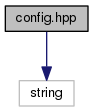
\includegraphics[width=142pt]{config_8hpp__incl}
\end{center}
\end{figure}
This graph shows which files directly or indirectly include this file\+:
\nopagebreak
\begin{figure}[H]
\begin{center}
\leavevmode
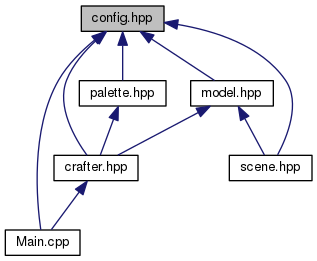
\includegraphics[width=310pt]{config_8hpp__dep__incl}
\end{center}
\end{figure}
\subsection*{Macros}
\begin{DoxyCompactItemize}
\item 
\#define {\bfseries M\+O\+D\+E\+L\+L\+I\+NG}~0\hypertarget{config_8hpp_ac1176ef1ef64f5125cbd690c61d7afdf}{}\label{config_8hpp_ac1176ef1ef64f5125cbd690c61d7afdf}

\item 
\#define {\bfseries I\+N\+S\+P\+E\+C\+T\+I\+ON}~1\hypertarget{config_8hpp_a2d8de8855e8fbc5d7d1cdfa532ebe545}{}\label{config_8hpp_a2d8de8855e8fbc5d7d1cdfa532ebe545}

\item 
\#define {\bfseries B\+U\+F\+F\+E\+R\+\_\+\+O\+F\+F\+S\+ET}(offset)~((G\+Lvoid$\ast$) (offset))\hypertarget{config_8hpp_a2789ab28bb84a9a9f553c45e4eedbdfd}{}\label{config_8hpp_a2789ab28bb84a9a9f553c45e4eedbdfd}

\end{DoxyCompactItemize}
\subsection*{Variables}
\begin{DoxyCompactItemize}
\item 
const int {\bfseries cft\+::screen\+\_\+width} = 1000\hypertarget{config_8hpp_ab8bf249761acc430dc01682ceb5b11ca}{}\label{config_8hpp_ab8bf249761acc430dc01682ceb5b11ca}

\item 
const int {\bfseries cft\+::screen\+\_\+height} = 1000\hypertarget{config_8hpp_ac27e7b16c0164556f3deedf4e66e5ffb}{}\label{config_8hpp_ac27e7b16c0164556f3deedf4e66e5ffb}

\item 
const int {\bfseries cft\+::screen\+\_\+depth} = 1000\hypertarget{config_8hpp_aec45f373686ae36a29dba598757a3d12}{}\label{config_8hpp_aec45f373686ae36a29dba598757a3d12}

\item 
const std\+::string {\bfseries cft\+::vertex\+\_\+shader} = \char`\"{}vertex\+\_\+shader.\+glsl\char`\"{}\hypertarget{config_8hpp_a7cd805c3372f0a7a7073fa9e7c34e6e6}{}\label{config_8hpp_a7cd805c3372f0a7a7073fa9e7c34e6e6}

\item 
const std\+::string {\bfseries cft\+::fragment\+\_\+shader} = \char`\"{}fragment\+\_\+shader.\+glsl\char`\"{}\hypertarget{config_8hpp_aacf92fa3cbf6fca965d9050d2729951f}{}\label{config_8hpp_aacf92fa3cbf6fca965d9050d2729951f}

\item 
const std\+::string {\bfseries cft\+::scene\+\_\+vertex\+\_\+shader} = \char`\"{}scene\+\_\+vertex\+\_\+shader.\+glsl\char`\"{}\hypertarget{config_8hpp_a55e7e5756c00c1b70fcb1d08bd5d6aad}{}\label{config_8hpp_a55e7e5756c00c1b70fcb1d08bd5d6aad}

\item 
const int {\bfseries cft\+::max\+\_\+vertices} = 500\hypertarget{config_8hpp_a1f4441e0e7e486d11acb518486d2dc3a}{}\label{config_8hpp_a1f4441e0e7e486d11acb518486d2dc3a}

\item 
const int {\bfseries cft\+::line\+\_\+gap} = 20\hypertarget{config_8hpp_a7a6abb1ed76dc5e8e758441f947ae240}{}\label{config_8hpp_a7a6abb1ed76dc5e8e758441f947ae240}

\item 
const float {\bfseries cft\+::delta\+\_\+rot} = 0.\+01\hypertarget{config_8hpp_a7598ed4ebb49298126495f63dc58b177}{}\label{config_8hpp_a7598ed4ebb49298126495f63dc58b177}

\item 
const float {\bfseries cft\+::delta\+\_\+trans} = 0.\+01\hypertarget{config_8hpp_aefd2a0ad35e04d11e5d2ba09de591b3e}{}\label{config_8hpp_aefd2a0ad35e04d11e5d2ba09de591b3e}

\item 
const float {\bfseries cft\+::camera\+\_\+x} = 0.\+0f\hypertarget{config_8hpp_a51f660b613928e7e778735c1e374ba3f}{}\label{config_8hpp_a51f660b613928e7e778735c1e374ba3f}

\item 
const float {\bfseries cft\+::camera\+\_\+y} = 0.\+0f\hypertarget{config_8hpp_a5cbf8645c529a7818b17f4cd566656a4}{}\label{config_8hpp_a5cbf8645c529a7818b17f4cd566656a4}

\item 
const float {\bfseries cft\+::camera\+\_\+z} = 3.\+0f\hypertarget{config_8hpp_ac09d9ddd6e18174031bbc4d2c27c8bcf}{}\label{config_8hpp_ac09d9ddd6e18174031bbc4d2c27c8bcf}

\item 
const float {\bfseries cft\+::xmin} = screen\+\_\+width -\/ 200.\+0f\hypertarget{config_8hpp_af4a44ec01e8868334c81eb5ea88c6061}{}\label{config_8hpp_af4a44ec01e8868334c81eb5ea88c6061}

\item 
const float {\bfseries cft\+::ymin} = 0.\+0f\hypertarget{config_8hpp_a1b82644d4edfed899f43f0c2f6ac5d26}{}\label{config_8hpp_a1b82644d4edfed899f43f0c2f6ac5d26}

\item 
const float {\bfseries cft\+::xmax} = screen\+\_\+width\hypertarget{config_8hpp_aa70c35ec80269dc749872e15e9603d39}{}\label{config_8hpp_aa70c35ec80269dc749872e15e9603d39}

\item 
const float {\bfseries cft\+::ymax} = 200.\+0f\hypertarget{config_8hpp_a0df139d99cc9012054fa0134a5edb657}{}\label{config_8hpp_a0df139d99cc9012054fa0134a5edb657}

\item 
const float {\bfseries cft\+::left} = -\/2.\+0\hypertarget{config_8hpp_a0be85df1e845da3ec4add0975dc69a43}{}\label{config_8hpp_a0be85df1e845da3ec4add0975dc69a43}

\item 
const float {\bfseries cft\+::right} = 2.\+0\hypertarget{config_8hpp_a335b6e470ad30d50b1b36cb79d8024ea}{}\label{config_8hpp_a335b6e470ad30d50b1b36cb79d8024ea}

\item 
const float {\bfseries cft\+::top} = -\/2.\+0\hypertarget{config_8hpp_adbef824162abfdc67afa23f0db5b7e45}{}\label{config_8hpp_adbef824162abfdc67afa23f0db5b7e45}

\item 
const float {\bfseries cft\+::bottom} = 2.\+0\hypertarget{config_8hpp_aa9b19490c250ba45ee22c9a8b4daad51}{}\label{config_8hpp_aa9b19490c250ba45ee22c9a8b4daad51}

\item 
const float {\bfseries cft\+::near} = -\/20.\+0\hypertarget{config_8hpp_a82c2d80f8c579e215b6e862cf2a3aa9e}{}\label{config_8hpp_a82c2d80f8c579e215b6e862cf2a3aa9e}

\item 
const float {\bfseries cft\+::far} = 20.\+0\hypertarget{config_8hpp_aa660a48a7a31b836e9193f80b4e5a589}{}\label{config_8hpp_aa660a48a7a31b836e9193f80b4e5a589}

\end{DoxyCompactItemize}


\subsection{Detailed Description}
This stores all constants required to run the Crafter for simplicity of modifying. 


\hypertarget{crafter_8hpp}{}\section{crafter.\+hpp File Reference}
\label{crafter_8hpp}\index{crafter.\+hpp@{crafter.\+hpp}}


Class declaration for the program managing the state and models.  


{\ttfamily \#include $<$G\+L/glew.\+h$>$}\\*
{\ttfamily \#include $<$G\+L\+F\+W/glfw3.\+h$>$}\\*
{\ttfamily \#include $<$iostream$>$}\\*
{\ttfamily \#include $<$string$>$}\\*
{\ttfamily \#include \char`\"{}shader\+\_\+util.\+hpp\char`\"{}}\\*
{\ttfamily \#include \char`\"{}config.\+hpp\char`\"{}}\\*
{\ttfamily \#include \char`\"{}model.\+hpp\char`\"{}}\\*
{\ttfamily \#include \char`\"{}palette.\+hpp\char`\"{}}\\*
Include dependency graph for crafter.\+hpp\+:
\nopagebreak
\begin{figure}[H]
\begin{center}
\leavevmode
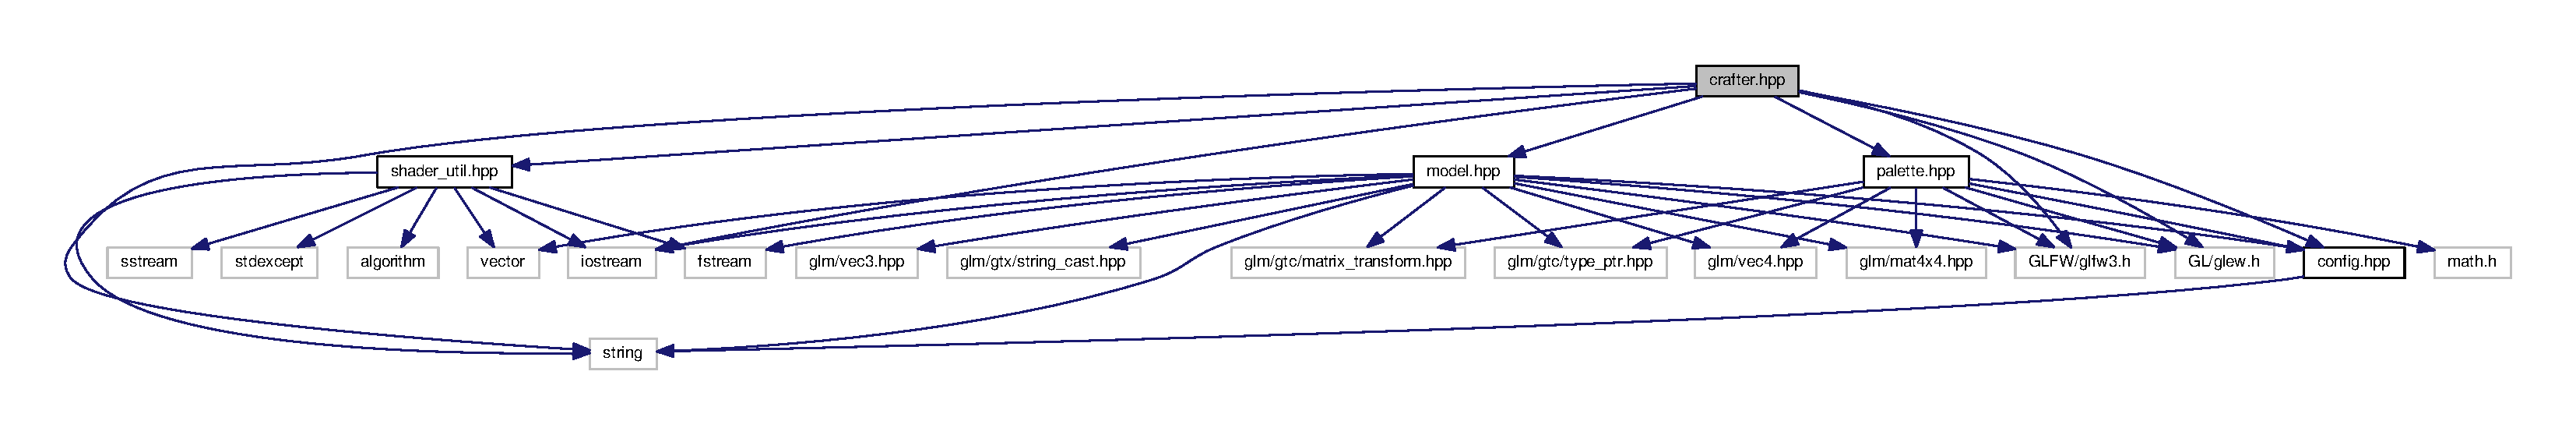
\includegraphics[width=350pt]{crafter_8hpp__incl}
\end{center}
\end{figure}
This graph shows which files directly or indirectly include this file\+:
\nopagebreak
\begin{figure}[H]
\begin{center}
\leavevmode
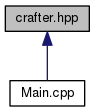
\includegraphics[width=143pt]{crafter_8hpp__dep__incl}
\end{center}
\end{figure}
\subsection*{Classes}
\begin{DoxyCompactItemize}
\item 
class \hyperlink{classcft_1_1Crafter}{cft\+::\+Crafter}
\begin{DoxyCompactList}\small\item\em Class that is basically the main program. \end{DoxyCompactList}\end{DoxyCompactItemize}


\subsection{Detailed Description}
Class declaration for the program managing the state and models. 


\hypertarget{Main_8cpp}{}\section{Main.\+cpp File Reference}
\label{Main_8cpp}\index{Main.\+cpp@{Main.\+cpp}}


Main funciton which creates and passes the window to the Crafter.  


{\ttfamily \#include $<$G\+L/glew.\+h$>$}\\*
{\ttfamily \#include $<$G\+L\+F\+W/glfw3.\+h$>$}\\*
{\ttfamily \#include $<$iostream$>$}\\*
{\ttfamily \#include \char`\"{}config.\+hpp\char`\"{}}\\*
{\ttfamily \#include \char`\"{}crafter.\+hpp\char`\"{}}\\*
Include dependency graph for Main.\+cpp\+:
\nopagebreak
\begin{figure}[H]
\begin{center}
\leavevmode
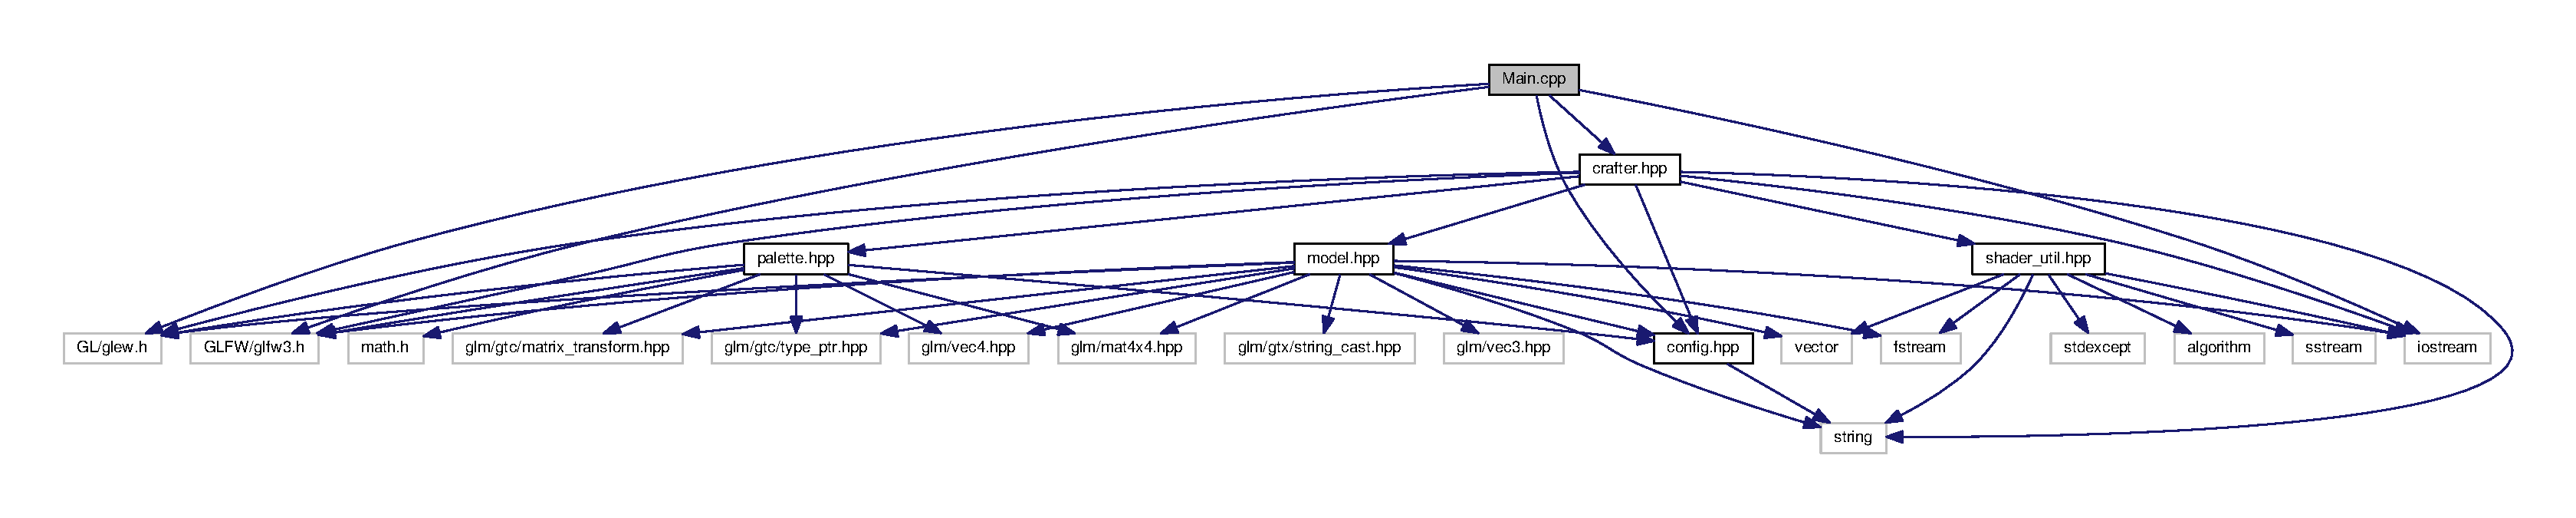
\includegraphics[width=350pt]{Main_8cpp__incl}
\end{center}
\end{figure}
\subsection*{Functions}
\begin{DoxyCompactItemize}
\item 
int {\bfseries main} ()\hypertarget{Main_8cpp_ae66f6b31b5ad750f1fe042a706a4e3d4}{}\label{Main_8cpp_ae66f6b31b5ad750f1fe042a706a4e3d4}

\end{DoxyCompactItemize}


\subsection{Detailed Description}
Main funciton which creates and passes the window to the Crafter. 


\hypertarget{model_8hpp}{}\section{model.\+hpp File Reference}
\label{model_8hpp}\index{model.\+hpp@{model.\+hpp}}


Class declaration for the Model.  


{\ttfamily \#include $<$iostream$>$}\\*
{\ttfamily \#include $<$string$>$}\\*
{\ttfamily \#include $<$vector$>$}\\*
{\ttfamily \#include $<$fstream$>$}\\*
{\ttfamily \#include $<$G\+L/glew.\+h$>$}\\*
{\ttfamily \#include $<$G\+L\+F\+W/glfw3.\+h$>$}\\*
{\ttfamily \#include \char`\"{}glm/vec3.\+hpp\char`\"{}}\\*
{\ttfamily \#include \char`\"{}glm/vec4.\+hpp\char`\"{}}\\*
{\ttfamily \#include \char`\"{}glm/mat4x4.\+hpp\char`\"{}}\\*
{\ttfamily \#include \char`\"{}glm/gtx/string\+\_\+cast.\+hpp\char`\"{}}\\*
{\ttfamily \#include \char`\"{}glm/gtc/matrix\+\_\+transform.\+hpp\char`\"{}}\\*
{\ttfamily \#include \char`\"{}glm/gtc/type\+\_\+ptr.\+hpp\char`\"{}}\\*
{\ttfamily \#include \char`\"{}config.\+hpp\char`\"{}}\\*
Include dependency graph for model.\+hpp\+:
% FIG 0
This graph shows which files directly or indirectly include this file\+:
% FIG 1
\subsection*{Classes}
\begin{DoxyCompactItemize}
\item 
class \hyperlink{classcft_1_1Model}{cft\+::\+Model}
\begin{DoxyCompactList}\small\item\em Class that is abstraction of a 3\+D-\/\+Model. \end{DoxyCompactList}\end{DoxyCompactItemize}


\subsection{Detailed Description}
Class declaration for the Model. 


\hypertarget{palette_8hpp}{}\section{palette.\+hpp File Reference}
\label{palette_8hpp}\index{palette.\+hpp@{palette.\+hpp}}


Class declaration for the Color Palette.  


{\ttfamily \#include $<$math.\+h$>$}\\*
{\ttfamily \#include $<$G\+L/glew.\+h$>$}\\*
{\ttfamily \#include $<$G\+L\+F\+W/glfw3.\+h$>$}\\*
{\ttfamily \#include \char`\"{}glm/vec4.\+hpp\char`\"{}}\\*
{\ttfamily \#include \char`\"{}glm/mat4x4.\+hpp\char`\"{}}\\*
{\ttfamily \#include \char`\"{}glm/gtc/matrix\+\_\+transform.\+hpp\char`\"{}}\\*
{\ttfamily \#include \char`\"{}glm/gtc/type\+\_\+ptr.\+hpp\char`\"{}}\\*
{\ttfamily \#include \char`\"{}config.\+hpp\char`\"{}}\\*
Include dependency graph for palette.\+hpp\+:
\nopagebreak
\begin{figure}[H]
\begin{center}
\leavevmode
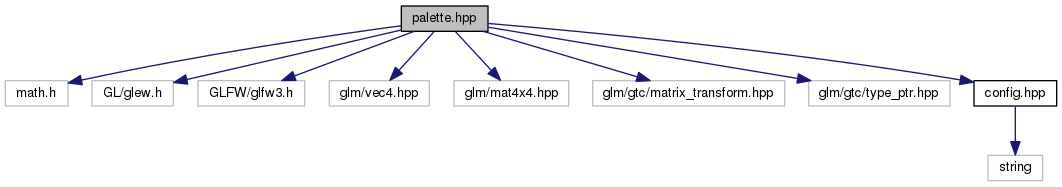
\includegraphics[width=350pt]{palette_8hpp__incl}
\end{center}
\end{figure}
This graph shows which files directly or indirectly include this file\+:
\nopagebreak
\begin{figure}[H]
\begin{center}
\leavevmode
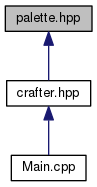
\includegraphics[width=145pt]{palette_8hpp__dep__incl}
\end{center}
\end{figure}
\subsection*{Classes}
\begin{DoxyCompactItemize}
\item 
class \hyperlink{classcft_1_1Palette}{cft\+::\+Palette}
\begin{DoxyCompactList}\small\item\em Class that displays a Rectangle Color-\/\+Palette to choose from. \end{DoxyCompactList}\end{DoxyCompactItemize}


\subsection{Detailed Description}
Class declaration for the Color Palette. 


%--- End generated contents ---

% Index
\backmatter
\newpage
\phantomsection
\clearemptydoublepage
\addcontentsline{toc}{chapter}{Index}
\printindex

\end{document}
